\section{Introduction}

Statistical methods for analyzing network data have become increasingly useful for studying  phenomenon ranging from people communicating online to protein interactions \cite{Goldenberg2009}.
One unifying idea is that the nodes of these networks are differentiated by rates of interacting with other parts of the network [TODO] that is associated with some other quantity, e.g. a covariate such as age or sex, or perhaps shared [TODO].
Stochastic blockmodels \cite{Nowicki2001, Kemp, Ishiguro2010, Rodriguez} are a class of statistical models for static network data that employ latent variables to model this heterogeneity by 1) assuming each node in the network belongs to some block (or cluster) and 2) parameterizing the probability of edges between nodes of each block. 

If we are interested in studying the events in a network, there are other aspects of the dynamics in addition to the mean rate. 
For example, human conversation often has an increased propensity for reciprocated events.
Shared tendencies based on other observed or unobserved quantities is of interest (who shares this tendency).
[TODO: Example of a shared dynamic... perhaps sticking with the reciprocity bit.]
Figure \ref{fig:introexample} shows how an analysis using a blockmodels will be unable to learn about these differences.

%A limitation of all of these approaches is the assumption of a single common behavior for all individuals.
%In contrast, in real-world networks it is reasonable to expect {\it heterogeneity} in dynamic behavior.  
%In an organization, the manner in which an individual communicates with others may be a function of an individual's {\it role} in the organization.
%For example, in a university,  email communication patterns over time between professors, students, and staff will likely be quite different within and between the three groups.

% - used to thinking about actors differentiated by rates
% - other things in the dynamics than rates, e.g. form of interaction.
% - Also important aspect of modeling social dynamics.
% especially important in cases like plot 1(c) where classical methods
% will fail.

%PS: not totally happy with this example since the "roles" are completely determined by one's "job title" and I think we would prefer something
% less explicit, e.g., that there are "leaders", "followers", etc, that go beyond just job titles. So feel free to edit this further!

%
%comprised of several teams, each team may uncover different patterns for collaborating via email---individuals in one group may respond more quickly, while another group may preferentially send to highly active individuals.

% TODO: Mention dynamic stochastic equivalence

Borrowing from the intuition of stochastic blockmodels, we propose a continuous-time model of network-based event sequences where latent clusters of nodes share similar patterns of interaction.
Our approach employs a flexible framework for  specifing how the process depends on the previous history of events \cite{AalenOddO.2008, Butts2008}.
%extend continuous-time models from event history analysis to model sequences of network-based event data \cite{Butts2008,Brandes2009,Perry2011,Stadtfeld2010,Stadtfeld2011,Opsahl2011,Vu2011,Vu2011a}. % \cite{AalenOddO.2008} 
%These models allow one to specify how the process depends on the previous history of events. % TODO use 'flexible'?
In this way one may investigate theories about the underlying processes and make predictions about future data conditioned on the past.

We describe parameter estimation and learning of  latent cluster assignments via MCMC, and illustrate the behavior of the model  with simulated data.
Using several real-world social network data sets involving dyadic communication, we compare the predictive performance of the fitted models to standard baselines.
Finally we show that the parameter estimates exhibit an interpretable structure to the event dynamics, enabling the study of a dynamic extension to stochastic equivalence.
%allowing identification of particular \emph{roles} in  that enable 

\begin{figure}
\centering
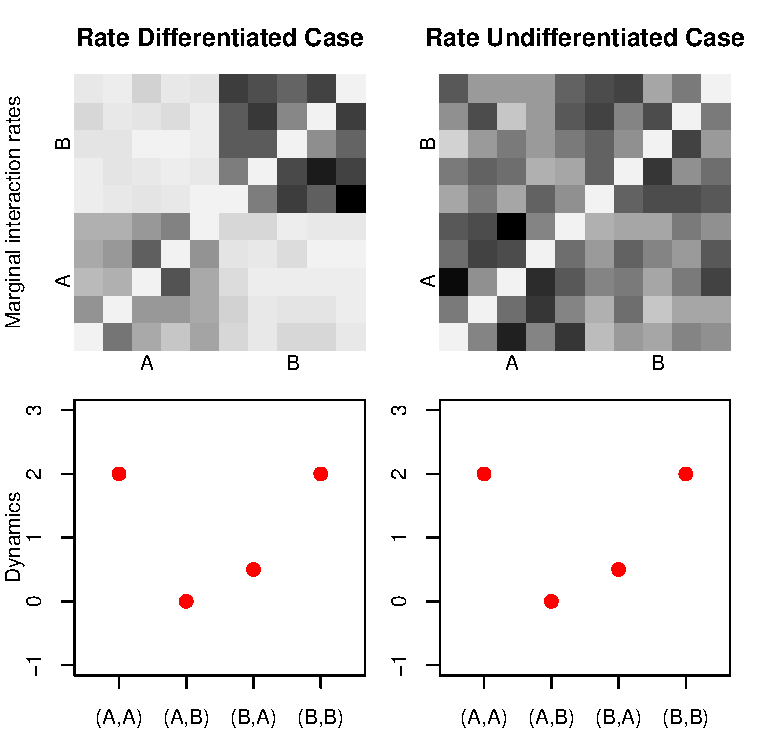
\includegraphics[scale=.8]{../figs/introexample/all}
\caption{}
\label{fig:example}
\end{figure}
